%!TEX program = xelatex
\documentclass[10pt]{article}
\usepackage{amssymb}
\usepackage{amsmath}
\usepackage{mathrsfs}
\usepackage{titlesec}
\usepackage{xcolor}
%\usepackage[shortlabels]{enumitem}
\usepackage{enumerate}
\usepackage{bm}
\usepackage{tikz}
\usepackage{listings}
\usetikzlibrary{arrows}
\usepackage{subfigure}
\usepackage{graphicx,booktabs,multirow}
\usepackage[a4paper]{geometry}
\usepackage{upquote}
\usepackage{float}
\usepackage{pdfpages}

\usepackage[colorlinks,linkcolor=blue]{hyperref}
\usepackage{mdframed}

\iffalse
\usepackage{lastpage}
\usepackage{fancyhdr}
\fancyfoot[C]{Page \thepage\ of \pageref{LastPage}}
% Uncomment to remove the header rule
\renewcommand{\headrulewidth}{0pt} 
\pagestyle{fancy}
\fi

\geometry{verbose,tmargin=2cm,bmargin=2cm,lmargin=2cm,rmargin=2cm}
\geometry{verbose,tmargin=2cm,bmargin=2cm,lmargin=2cm,rmargin=2cm}
\lstset{language=Matlab}
\lstset{breaklines}

\input defs.tex

\newenvironment{solution}
    { \begin{mdframed}[backgroundcolor=gray!10] \textcolor{cyan}{\textbf{Solution}} \\}
    {  \end{mdframed}}

\newtheorem{proposition}{Proposition}
\newtheorem{remark}{Remark}

\titleformat*{\section}{\centering\LARGE\scshape}
\renewcommand{\thesection}{\Roman{section}}
\lstset{language=Matlab,tabsize=4,frame=shadowbox,basicstyle=\footnotesize,
keywordstyle=\color{blue!90}\bfseries,breaklines=true,commentstyle=\color[RGB]{50,50,50},stringstyle=\ttfamily,numbers=left,numberstyle=\tiny,
  numberstyle={\color[RGB]{192,92,92}\tiny},backgroundcolor=\color[RGB]{245,245,244},inputpath=code}

\begin{document}

\title{CS150: Database and Data Mining \\%
	Final Exam Solution}
\maketitle


\section{ \textbf{ SQL and Relational Algebra [14 points]}}

You want to use your SQL skills to infer what is happening during the Battle of Hogwarts, and you could assume you have the following tables:
\\
\\
\\
CREATE TABLE Wizards(wizid integer, name text, house text, evil boolean, PRIMARY KEY(wizid));
\\
\\
CREATE TABLE Spells(sid integer, name text, offensive boolean, PRIMARY KEY (sid));
\\
\\
CREATE TABLE Attacks(attackid integer, attacker integer, attacked integer, spell integer,\\
PRIMARY KEY (attackid), FOREIGN KEY(spell) REFERENCES Spells,\\
FOREIGN KEY(attacker) REFERENCES Wizards, FOREIGN KEY(attacked) REFERENCES Wizards);
\\
\\
\\
\textbf{Note}: For all of the following questions, you do not need any Harry Potter knowledge. Any understanding of Wizards or Spells will not be helpful.
\begin{enumerate}
    \item (2 points) Select all of the following queries that return the name of each wizard who has been an
attacker more than 3 times. Do not assume that names are unique.\\
    \begin{enumerate}
        {\color{red}\item SELECT name FROM Wizards, Attacks\\
WHERE wizid = attacker\\
GROUP BY attacker, name\\
HAVING COUNT(*) \textgreater  3;\\}
    \item SELECT name FROM Wizards, Attacks\\
WHERE wizid = attacker\\
GROUP BY name\\
HAVING COUNT(*) \textgreater 3;\\
    {\color{red}\item SELECT name FROM\\
    \quad (SELECT name FROM Wizards, Attacks\\
\quad\quad WHERE wizid = attacker) AS a\\
GROUP BY attacker,name\\
HAVING COUNT(*) \textgreater 3\\
ORDER BY COUNT(name);\\}
    \\

    \end{enumerate}
    \item (2 points) Select all of the following queries that select the names of wizards (A) that another individual
wizard (B) attacked twice, where the attacker (B) used two different spells. There should be no duplicates
in this list. Do not assume that names are unique.\\
\begin{enumerate}
    \item SELECT w1.name AS A\\
FROM Wizards w1, Wizards w2, Attacks a1, Attacks a2\\
WHERE w1.wizid = a1.attacked AND a1.spell != a2.spell\\
AND w2.wizid = a2.attacked AND a1.attacked = a2.attacked;\\
\item SELECT DISTINCT w1. name AS A\\
FROM Wizards w1, Attacks a1, Attacks a2\\
WHERE w1.wizid = a1.attacked AND a1.spell != a2.spell\\
AND w1.wizid = a2.attacked AND a1.attacked = a2.attacked;\\
{\color{red}\item SELECT DISTINCT w1.name AS A\\
FROM Wizards w1, Wizards w2, Attacks a1, Attacks a2\\
WHERE a1.attacker = a2.attacker AND w1.wizid = a1.attacked\\
AND a1.spell != a2.spell AND w2.wizid = a2.attacked AND a1.attacked = a2.attacked;\\}
\end{enumerate}
\item  (2 points) Select all of the following queries that return the name of all of the spells that have never
been used in an attack.\\
\begin{enumerate}
    {\color{red}\item SELECT name\\
FROM Spells\\
WHERE sid NOT IN\\
(SELECT spell FROM Attacks);\\}
{\color{red}\item SELECT name\\
FROM Spells\\
WHERE NOT EXISTS\\
(SELECT * FROM Attacks WHERE spell = sid);\\}
\item SELECT Spells.name\\
FROM Spells, Wizards, Attacks\\
WHERE wizid = attacker and spell = sid;\\
\end{enumerate}
\end{enumerate}
Fill in the following blanks to create a query that returns true if more evil wizards cast offensive spells, and returns false if more good wizards cast offensive spells.\\
\textbf{Note}: there could be more than one correct answer(s).\\
\\
\\
WITH countEevilGoodSpells(evil, numOffensive) AS\\
(SELECT  evil, count(*)\\
FROM  attacks, wizards, spells\\
WHERE  \underline{\quad\quad1\quad\quad} and spell = sid\\
AND offensive = \underline{\quad\quad2\quad\quad}\\
GROUP BY \underline{\quad\quad3\quad\quad})\\
SELECT evil\\
FROM countEevilGoodSpells\\
WHERE numOffensive $\ge$ ALL\\
(SELECT numOffensive\\
FROM \underline{\quad\quad4\quad\quad});\\
\\
\begin{enumerate}
    \item (1 points) Fill in the blank labeled (1).
    \begin{enumerate}
        \item wizid=attackid
        \item wizid=attacked
        {\color{red}\item wizid=attacker}
    \end{enumerate}
    \item (1 points) Fill in the blank labeled (2).
    \begin{enumerate}
        {\color{red}\item True}
        \item False
    \end{enumerate}
    \item (1 points) Fill in the blank labeled (3).
    \begin{enumerate}
        {\color{red}\item evil}
        \item spell
        \item attacker
    \end{enumerate}
    \item (1 points) Fill in the blank labeled (4).
    \begin{enumerate}
        \item Wizards
        {\color{red}\item countEevilGoodSpells}
        \item Attacks
    \end{enumerate}
    \item (2 points) Select all of the following answers that return the wizid of all of the wizards who have not
attacked anybody.
\begin{enumerate}
    \item $\pi_{\text {wizid }}(  Attacks  -  Wizards)$
    {\color{red}\item $\pi_{w i z i d}\left(\pi_{w i z i d}(W i z a r d s)-\pi_{a t t a c k e r}(  Attacks )\right) $}
    {\color{red}\item $\pi_{\text {wizid }}(  Wizards  )-\pi_{\text {attacker }}\left(\right.  Spells  \bowtie_{\text {sid }=  spell } Attacks  \bowtie_{\text {attacker }=  wizid} Wizards)$}
    \item $\pi_{\mathrm{wizid}, \text { name }}  (Wizards)  -\pi_{\mathrm{attacker}}  (Attacks)$\\
\end{enumerate}
\item (2 points) Select all of the following answers that return the wizid of all of the wizards who were
attacked by Wizards whose house is Gryffindor.
\begin{enumerate}
    {\color{red}\item $\pi_{\text {attacked }}\left(\right.  Spells  \bowtie_{\text {sid }=  spell} Attacks  \bowtie_{\text {attacker }=  wizid}  \sigma_{\text {house }=  'Gryffindor'} (Wizards  \left.)\right) $}
    \item $\pi_{\text {attacked }}\left(\right.  Spells  \bowtie_{\text {sid }=  spell} Attacks  \bowtie_{\text {attacker }=  wizid } \sigma_{\text {house }=  Gryffindor' } \left(\pi_{\text {wizid }}((\right.  Wizards  \left.))\right) $
    
    \item $\pi_{\text {wizid }}(W i z a r d s)-\pi_{\text {attacked }}\left(\right.  Spells  \bowtie_{\text {sid }=  spell } Attacks  \bowtie_{\text {attacked }=  wizid } \sigma_{\text {house } !=' G r y f f i n d o r '}   (Wizards  \left.)\right) $
    
    \item $\pi_{\text {attacked }}\left(\right.  Attacks  \bowtie_{\text {attacker }=\text { wizid }}\left(\sigma_{\text {house }=' G r y f f i n d o r ' } (  Wizards  ) \bowtie_{\text {sid }=\text { spell }}  Spells  \left.)\right) $
\end{enumerate}
\end{enumerate}
\quad\par
\quad\par
\quad\par
\quad\par
\quad\par


\newpage



\section{ \textbf{B+ Trees [10 points]}}
Given the following (degree d = 1) B+ tree:
\begin{figure}[h]\centering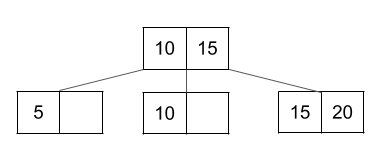
\includegraphics[height=3cm]{b+tree.png}\end{figure}\\
\begin{enumerate}
    \item[(a)] [6 points] Draw what the tree looks like after adding 2, 6, and 12 in that order.\\ \begin{figure}[h]\centering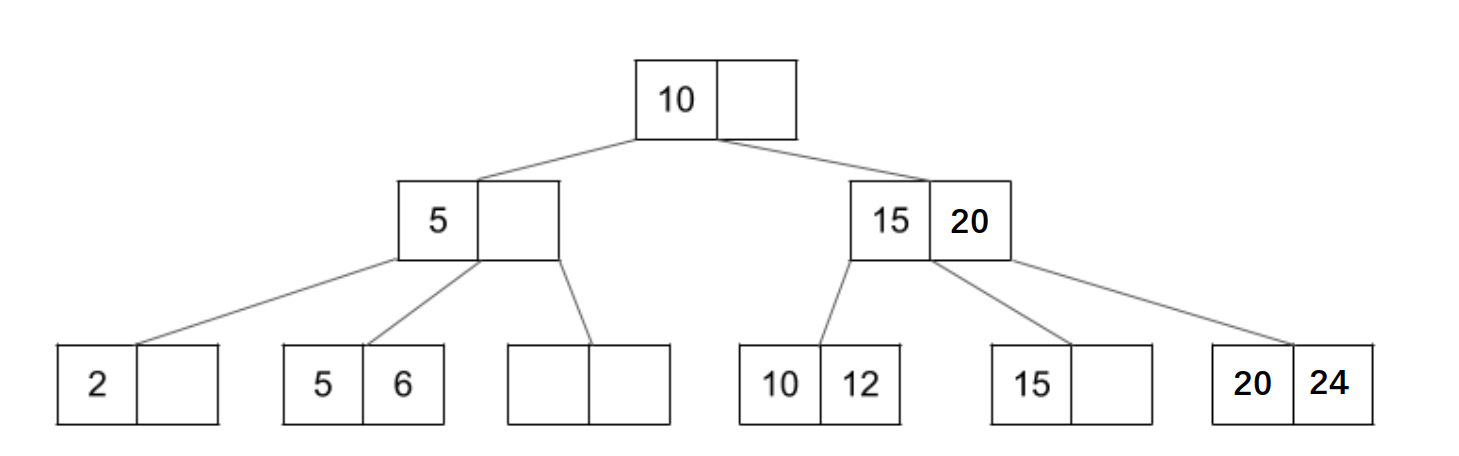
\includegraphics[height=3.5cm]{b+tree_sol.png}\end{figure}
\end{enumerate}\\

\noindent For the following questions, consider the tree directly after 2, 6, and 12 have been added.
\begin{enumerate}
    \item[(b)] [2 points] What is the maximum number of inserts we can do without changing the height of the tree?\\ 
    {\color{red} Answer: 10 inserts. \\ The maximum number of keys for a fixed height h is given by 2d · (2d + 1)h.
    We have d = 1 from the question, and h = 2 (we must remember h is the number of non-root layers).
    Plugging these numbers in gives us 2 ∗ 32 = 18.\\
    Now, we already have 8 keys in the tree, so we can insert 18 − 8 = 10 more.}
 \item[(c)][2 points] What is the minimum number of inserts we can do that will change the height of the tree?\\ {\color{red} Answer: 3 inserts (e.g. 25, 26, 27).
The idea is to repeatedly insert into the fullest nodes; this is hopefully apparent from understanding
how and when B-trees split.}
\end{enumerate}
% Given the following (degree d = 1) B+ tree:\\
% 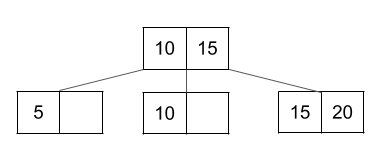
\includegraphics[height=3cm]{b+tree.png}\\
% (a)[6 points] Draw what the tree looks like after adding 2, 6, and 12 in that order.\\
% 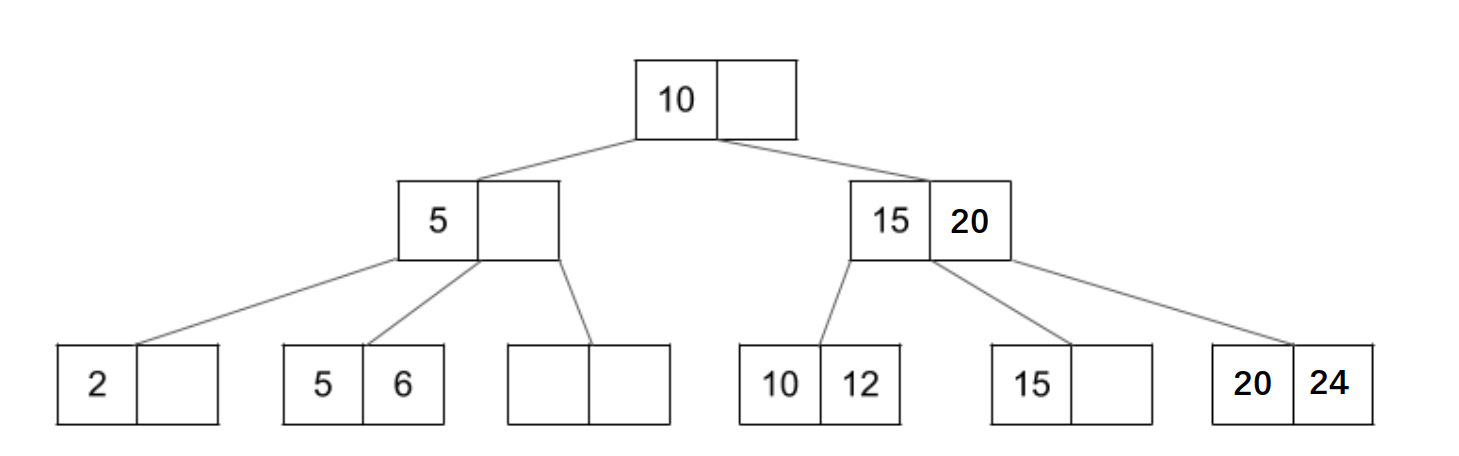
\includegraphics[height=3.5cm]{b+tree_sol.png}
% \\
% \\
% For the following questions, consider the tree directly after 2, 6, and 12 have been added.\\
% \\
% (b)[2 points] What is the maximum number of inserts we can do without changing the height of the tree?\\
% \\
% {\color{red} Answer: 10 inserts. The maximum number of keys for a fixed height h is given by 2d · (2d + 1)h.
% We have d = 1 from the question, and h = 2 (we must remember h is the number of non-root layers).
% Plugging these numbers in gives us 2 ∗ 32 = 18.\\
% Now, we already have 8 keys in the tree, so we can insert 18 − 8 = 10 more.}\\
% \\
% (c)[2 points] What is the minimum number of inserts we can do that will change the height of the tree?\\
% \\
% {\color{red} Answer: 3 inserts (e.g. 25, 26, 27).
% The idea is to repeatedly insert into the fullest nodes; this is hopefully apparent from understanding
% how and when B-trees split.}


% \newpage

\section{\textbf{Buffer Management and Relational Algebra [12 points]}}
\begin{enumerate}
    \item[1.] [8 points] We’re given a buffer pool with 4 pages, which is empty to begin with. Answer the following questions given
this access pattern:
\begin{center}
A B C D E B A D C A E C
\end{center}
\begin{enumerate}
    \item[(a)] [4 points] What is the hit rate for LRU? {\quad\color{red}Answer: 4/12}
    \item[(b)][4 points] In order of when they were first placed into the buffer pool, what pages remain in the buffer pool after this sequence of accesses?{\quad\color{red}Answer: C E A D}
\end{enumerate}
    \item[2.] [4 points] Consider two relations with the same schema: R(A,B,C) and S(A,B,C). Which one of the following relational
algebra expressions is not equivalent to the others?
\begin{enumerate}
\item[(A)] $\pi_{R.A}((R\cup S)-S)$
\item[(B)] $\pi_{R.A}(R)-\pi_{R.A}(R\cap S)$
\item[(C)] $\pi_{R.A}(R-S)\cap \pi_{R.A}(R)$
\item[(D)] $\pi_{R.A}(R-S)$
\end{enumerate}
{\color{red} Answer: B. Consider the counter example where R(A, B) = (1,2), (1,3) and S(A, B) = (1,2). a and c
will result in a size 1 set, while b will result in a size 0 set.}
\end{enumerate}
% 1.[4 points] We’re given a buffer pool with 4 pages, which is empty to begin with. Answer the following questions given
% this access pattern:
% \begin{center}
% A B C D E B A D C A E C
% \end{center}
% (a)[4 points] What is the hit rate for LRU?\\
% {\color{red}Answer: 4/12}
% \\
% \\
% (b)[4 points] In order of when they were first placed into the buffer pool, what pages remain in the buffer pool after
% this sequence of accesses?\\
% {\color{red}Answer: C E A D}
% \\
% \\
% \\
% \\
% 2. [4 points] Consider two relations with the same schema: R(A,B,C) and S(A,B,C). Which one of the following relational
% algebra expressions is not equivalent to the others?\\
% (A)$\pi_{R.A}((R\cup S)-S)$\\
% (B)$\pi_{R.A}(R)-\pi_{R.A}(R\cap S)$\\
% (C) $\pi_{R.A}(R-S)\cap \pi_{R.A}(R)$\\
% (D) $\pi_{R.A}(R-S)$\\
% \\
% {\color{red} Answer: B. Consider the counter example where R(A, B) = (1,2), (1,3) and S(A, B) = (1,2). a and c
% will result in a size 1 set, while b will result in a size 0 set.}


% \newpage

\section{ \textbf{External Sorting and Hashing [18 points]}}

\begin{itemize}
    \item True or False (2 points)
    \begin{enumerate}
        \item  Increasing the number of buffer pages does not affect the number of I/Os performed in Pass 0\\
        \\
        {\color{red}Solution: True. Regardless of the number of buffer pages, every pass of an external sort (including Pass 0) performs the same number of IOs.
of an external sort.\\}
        \item Double buffering reduces the time it takes to sort records within a single page.\\
        \\
        {\color{red}Solution: False. Double buffering allows a program to concurrently perform computations and fetch data from disk. Once a page of data is resident in memory, double buffering will not help speed up computation on it.}
    \end{enumerate}
    \quad\par \quad\par 
    \item Let’s Sort and Hash This Out! (16 points)
    \\
    \\
    Now you're facing the problem of figuring out the steps to sort a table in your DBMS. Assume your table is 100 pages and you have 5 buffer pages in memory. Please fill out the following pass-by-pass guide that details the number and the length of runs created after each pass in External Merge Sort.
    \\
    \\
    In the \textbf{second} blank for each pass, write all unique run lengths in \textbf{increasing} order, separated by commas. In the \textbf{first} blank for each pass, write the number of runs corresponding to each run length specified in the
second blank, separated by commas.\\ \\
For example, if there were 3 runs of length 50 created after Pass 0, then write 3 for the first blank and 50
for the second blank on the line for Pass 0.
If instead there were 6 runs created in total: 2 runs of length 10, 1 run of length 25, and 3 runs of length
50, then write 2, 1, 3 for the first blank and 10, 25, 50 for the second blank. \\ \\
    If the algorithm terminates before the last pass, write 0 for all blanks in unused passes. \\
    \begin{enumerate}
        \item Fill out the numbers for each blank in the following passes. (5 points)\\
        \begin{itemize}
            \item Pass 0: \underline{\quad\quad{\color{red}20}\quad\quad} run(s) of \underline{\quad\quad{\color{red}5}\quad\quad} page(s) are created.\\
            \item Pass 1: \underline{\quad\quad{\color{red}5}\quad\quad} run(s) of \underline{\quad\quad{\color{red}20}\quad\quad} page(s) are created.\\
            \item Pass 2: \underline{\quad\quad{\color{red}1,1}\quad\quad} run(s) of \underline{\quad\quad{\color{red}20,80}\quad\quad} page(s) are created.\\
            \item Pass 3: \underline{\quad\quad{\color{red}1}\quad\quad} run(s) of \underline{\quad\quad{\color{red}100}\quad\quad} page(s) are created.\\
            \item Pass 4: \underline{\quad\quad{\color{red}0}\quad\quad} run(s) of \underline{\quad\quad{\color{red}0}\quad\quad} page(s) are created.\\ \\
        \end{itemize}
        \item Based on the guide, how many I/Os does the entire External Merge Sort on this table take? (2 points)
        \\
        \\
        {\color{red}Solution: 800 (Using External Merge Sort formula: $2 N\left(1+\left\lceil\log _{B-1}\left\lceil\frac{N}{B}\right\rceil\right\rceil\right)=2 * 100 * ( 1 + \\
        \left.\left.\left\lceil\log _{4}\left\lceil\frac{100}{5}\right\rceil\right\rceil\right)=800\right)$\\
Full credit was also awarded to 760 if the student noticed that the run of 20 created after pass 2 is not merged so it doesn’t need to be read or written in that pass, saving 20 + 20 = 40 I/Os.}
        \\
    \end{enumerate}
    Now you also want to hash the table 
 which requires an exhaustive of the hashing process as well. Still assuming table is 100 pages and you have 5 buffer pages in memory, please fill out the following guide which details the number and size of partitions created after each partitioning pass in External Hashing. You could assume uniform hash functions are used in each pass.\\ \\
 In the \textbf{first} blank for each pass, write the total number of partitions created after the pass. In the \textbf{second}
blank, write the number of pages in each of those partitions. If not all partition passes are needed, write 0
for all blanks in unneeded passes.\\ \\
    \begin{enumerate}
        \item Fill out the numbers for each blank in the following passes. (5 points)\\
        \begin{itemize}
            \item Partitioning Pass 1: \underline{\quad\quad{\color{red}4}\quad\quad} partition(s) of \underline{\quad\quad{\color{red}25}\quad\quad} page(s) are created.\\
            \item Partitioning Pass 2: \underline{\quad\quad{\color{red}16}\quad\quad} partition(s) of \underline{\quad\quad{\color{red}7}\quad\quad} page(s) are created.\\
            \item Partitioning Pass 3: \underline{\quad\quad{\color{red}64}\quad\quad} partition(s) of \underline{\quad\quad{\color{red}2}\quad\quad} page(s) are created.\\
            \item Partitioning Pass 4: \underline{\quad\quad{\color{red}0}\quad\quad} partition(s) of \underline{\quad\quad{\color{red}0}\quad\quad} page(s) are created.\\
            \item Partitioning Pass 5: \underline{\quad\quad{\color{red}0}\quad\quad} partition(s) of \underline{\quad\quad{\color{red}0}\quad\quad} page(s) are created.\\ \\
        \end{itemize}
        \item  Based on the guide, how many I/Os does the entire External Hashing process on this table
take? Remember that External Hashing consists of both the divide phase and the conquer phase. (4 points)
        \\
        \\
{\color{red}Solution: 908 \\
I/Os: (I/Os are in bold) In the 1st partitioning pass we read 100 pages and write 100 pages (4 partitions of 25 pages each). In the 2nd partitioning pass we read 100 pages and write 112 pages (16 partitions of 7 pages each). In the 3rd partitioning pass we read 112 pages and write 128 pages (64 partitions of 2 pages each). Now, we can build the hash tables which involves reading 128 pages and writing 128 pages. Adding all I/Os results in 908 I/Os.}
        \\
    \end{enumerate}
\end{itemize}


% \newpage


\section{\textbf{Iterators and Joins    [6 points]}}
Consider a case that, $B > 4$ pages worth of buffer space, and relations M and N of size $> B$. Please fill the blanks below with "always", "sometimes", or "never".
\begin{enumerate}
    \item[(a)] [2 points] Block nested loop join is \underline{\quad\quad\quad\quad} better than page-oriented nested loop join.\\
        {\color{red} Answer: Always. Block nested loop join is page-oriented on steroids, and steroids and always good.}
    \item[(b)] [2 points] Sort-merge join is \underline{\quad\quad\quad\quad} better than hash-join.\\
        {\color{red} Answer: Sometimes. Hash join is cooler if one relation is really small and one is very large. Sort dominates if you have lots of dumlicated join keys.}
    \item[(c)] [2 points] Hybrid Hash-Join is \underline{\quad\quad\quad\quad} better than block-nested loops join.\\
        {\color{red} Answer: Sometimes. Nested loops works for non-equijoins and hash does not. For equijoins, hash is often better since it only makes a small number of passes over each relation, whereas block nested-loops still may visit the inner relation many times. If one relation fits in memory, the two algorithm are about equivalent.}
\end{enumerate}




\newpage


\section{ \textbf{Query Optimization  [10 points]}}
Assume the following:
\begin{itemize}
    \item Column values are uniformly distributed and independent from one another
    \item Use System R defaults (1/10) when selectivity estimation is not possible
    \item Primary key IDs are sequential, starting from 1
    \item Our optimizer \textbf{does not consider interesting orders}
\end{itemize}
We have the following schema:
% \\
% Consider three relations Student(sid, b) and S(a), with 1000 tuples and 500 tuples respectively. We have
% an index on R.a with 50 unique integer values uniformly distributed in the range [1, 50], and an index on
% S.a with 25 unique integer values uniformly distributed in the range [1, 25]. We do not have an
% index on R.b.\\
\begin{figure}[h]\centering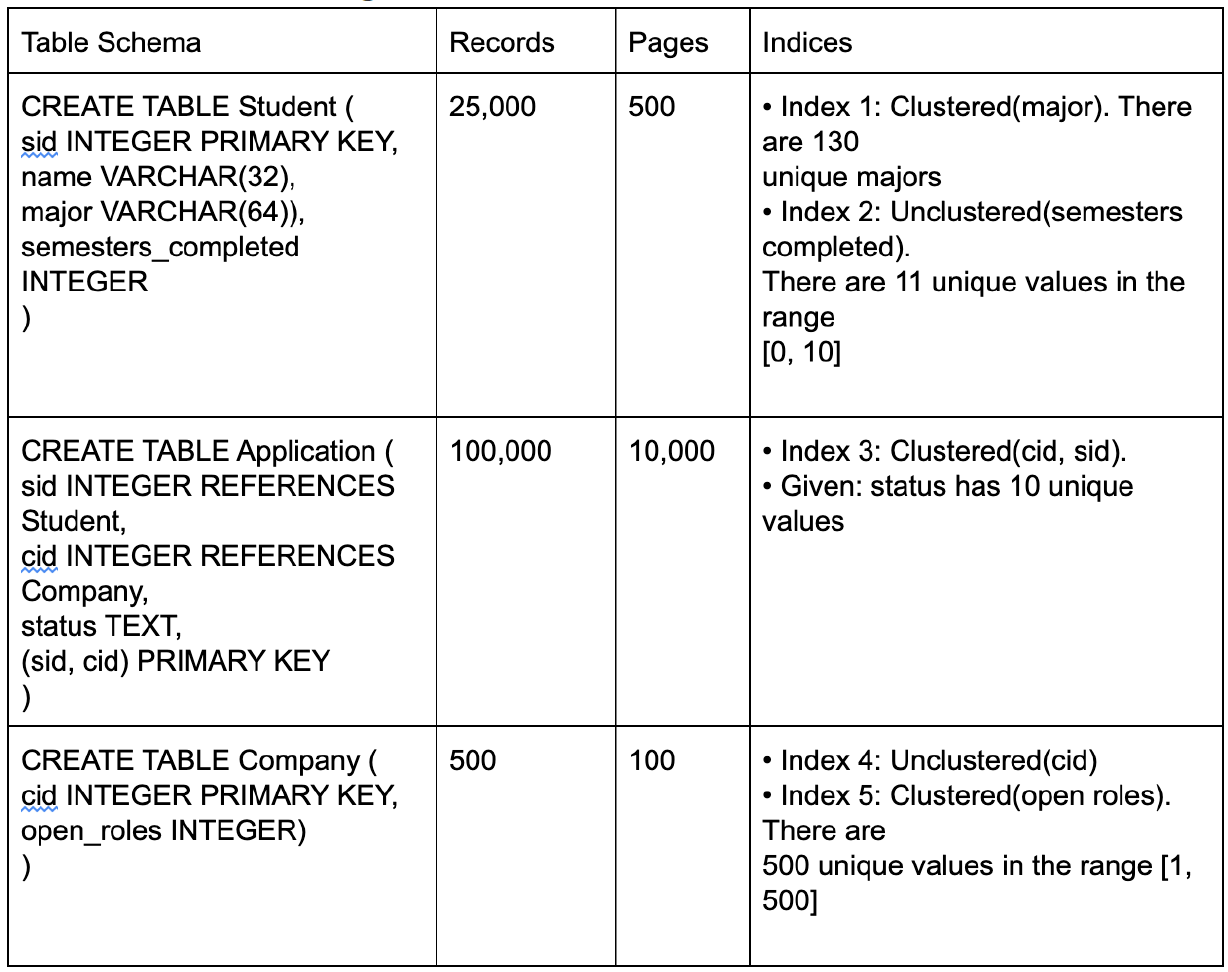
\includegraphics[height=8cm]{query_opt.png}\end{figure}\\
Consider the following query:\\
SELECT Student.name, Company.open\_roles, Application.referral\\
FROM Student, Application, Company\\
WHERE Student.sid = Application.sid \hfill -- (Selectivity 1)\\
% AND Application.cid = Company.cid  \hfill -- (Selectivity 2)\\
AND Student.semesters\_completed $>$ 4 \hfill -- (Selectivity 2)\\
AND (Student.major='CS' OR Company.open\_roles $<=$ 50) \hfill -- (Selectivity 3)\\
% AND NOT Application.status = 'limbo' \hfill -- (Selectivity 4)\\
ORDER BY Company.open\_roles;
\begin{enumerate}
    \item[1.] [4 points] For the following questions, calculate the selectivity of each of the labeled Selectivities above.
    \begin{enumerate}
        % \item Selectivity 1 \\ \\
        \item Selectivity 2 \\ 
        {\color{red}  (10 - 4) / (10 - 0 + 1) = 6/11.\\
        We have 11 unique values, assumed to be equally distributed. Therefore we use the equation for less than or equal to which is (high key - value) / (high key - low key + 1).}
        \item Selectivity 3 \\ 
        {\color{red}
        Sel(Student.major='CS') = 1/distinct values = 1/130\\
        Sel(Company.open\_roles $<=$ 50) = (v - low key) / ((high key - low key + 1) + (1 / number distinct)) = (50-1) / (500-1+1) + 1/500 = 1/10\\
        Selectivity 3 = S(p1) + S(p2) - S(p1)S(p2) = (1/130 + 1/10) - (1/130 * 1/10) = 10/1300 + 130/1300 - 1/1300 = 139/1300. }
    \end{enumerate}
    \item[2.] [6 points]  For each predicate, which is the first pass of Selinger's algorithm that uses its selectivity to estimate output size? (\textbf{Pass 1, 2 or 3}?)
    \begin{enumerate}
        \item Selectivity 1: \\
        $\square$ Pass 1 \quad {\color{red}$\checkmark$ Pass 2} \quad $\square$ Pass 3
        % \item Selectivity 2 \\
        % $\square$ Pass 1 \quad $\square$ Pass 2 \quad $\square$ Pass 3
        \item Selectivity 2 \\
        {\color{red}$\checkmark$ Pass 1} \quad $\square$ Pass 2 \quad $\square$ Pass 3
        \item Selectivity 3 \\
        $\square$ Pass 1 \quad $\square$ Pass 2 \quad {\color{red}$\checkmark$ Pass 3}
        % \item Selectivity 5 \\
        % $\square$ Pass 1 \quad $\square$ Pass 2 \quad $\square$ Pass 3
    \end{enumerate}
    {\color{red} (b) is pass 1 because they only involve filtering one table. \\
    (a) is pass 2 because they represent a join. \\
    Note that (c), the OR predicate, is over 2 tables that have no associated join predicate, so the selection is postponed along with the cross-product, until after 3-way joins are done.}
\end{enumerate}

% \newpage



\section{ \textbf{Concurrency Control  [10 points]}}
\begin{figure}[h]\centering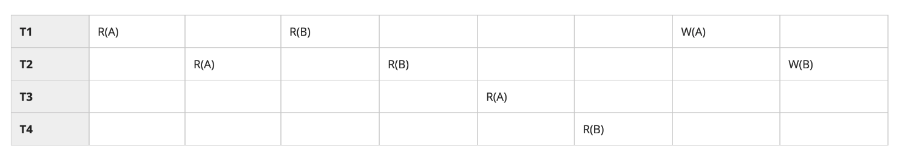
\includegraphics[height=2.5cm]{conflict.png}\end{figure}
\begin{enumerate}
    \item[(a)] [6 points] Draw the conflict dependency graph for the schedule.\\
\begin{center}
    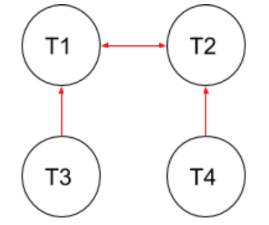
\includegraphics[height=3cm]{conflict_sol.png}
\end{center}
    \item[(b)] [4 points] Is this schedule conflict serializability? If so, write down all the conflict equivalent serial schedules. If not, explain the reason. \\
    {\color{red}  No, there's a cycle between T1 and T2. T1 must come before T2 and T2 before T1. Thus the schedule does not conflict serializable.}
\end{enumerate}
% (a)[6 points] Draw the conflict dependency graph for the schedule.

% (b)[4 points] Is this schedule conflict serializability? If so, write down all the conflict equivalent serial schedules? If not,explain the reason.\\

\section{ \textbf{Recovery [8 points]}}
% \quad\par
% \quad\par
% \quad\par
 For the following statements, please answer whether it is True or False. (8 points)

\begin{enumerate}
    \item When a transaction commits, any modified buffer pages must be written to durable storage.
    \\
    {\color{red}False. ARIES uses a NO FORCE policy.}
    \item When aborting a transaction, it may be necessary to modify pages on disk.
    \\
    {\color{red}True. ARIES uses a STEAL policy.}
    \item During recovery, the ARIES protocol may redo aborted transactions.
    \\
    {\color{red}True. This is a key feature of ARIES and essential for the correctness of the protocol.}
    \item The pageLSN contains the LSN of the last operation to modify the page.
    \\
    {\color{red}True. This is the definition of the pageLSN.}
    \item The tail of the log is always flushed after every update operation.
    \\
    {\color{red}False. We only require that the tail of the log be flushed on commit. Remember that flushedLSN keeps
track of the log tail.}
    \item A system that uses a FORCE, STEAL policy does not need to undo any operations after a crash.
    \\
    {\color{red}False. A system with a STEAL policy needs UNDO logging to ensure atomicity.}
    \item The recovery manager is responsible for Atomicity and Durability, as defined by the ACID acronym.
    \\
    {\color{red}True.}
    \item During a transaction abort, we redo all updates made by the transaction.
    \\
    {\color{red}False.}
\end{enumerate}


\newpage

\section{\textbf{FDs and BCNF [8 points]}}
\begin{enumerate}
    \item[1.] [4 points] Decompose $R=ABCDEFGH$ into BCNF in the order of the given functional dependencies: $F=\{ C\rightarrow A, B\rightarrow EF, H\rightarrow BCG, F\rightarrow CD, G\rightarrow B\}$.\\
    Select all the following tables included in the final decomposition.
    \begin{enumerate}
        \item AC
        \item BCDGH
        \item BCGH
        \item BG
        \item DH
    \end{enumerate}
    {\color{red} Answer: ADE\\
    $C\rightarrow A$: ABCDEFGH decomposes into BCDEFGH and AC\\
    $B\rightarrow EF$: BCDEFGH decomposes into BCDGH and BEF\\
    $H\rightarrow BCG$: BCDGH decomposes into DH and BCGH\\
    $F\rightarrow CD$: skip\\
    $G\rightarrow B$: BCGH decomposes into CGH and BG\\
    Final decomposition: AC, BEF, BG, CGH, DH}
    \item[2.] [4 points] Two students are writing a decomposition of tables based on the attributes set $R=ABCDEF$ and the functional dependency set $F=\{ C\rightarrow D, A\rightarrow B, B\rightarrow EF, F\rightarrow A \}$.\\
    Another student decides to write a decomposition of tables as $ABDE$ and $ABCF$. Right now, this is not a lossless decomposition. Which of the following changes (applied individually, not combined together) would make this a lossless decomposition?
    \begin{enumerate}
        \item Adding $D \rightarrow ABCDEF$ to the functional dependency set F.
        \item Adding $E \rightarrow C$ to the functional dependency set F.
        \item Adding $B \rightarrow D$ to the functional dependency set F.
    \end{enumerate}
     {\color{red} Answer: BC.\\
     The intersection is $AB \rightarrow ABEF$. To be lossless, either $AB \rightarrow ABDE$ or $AB \rightarrow ABCF$}
\end{enumerate}



\section{ \textbf{Parallel Querying  [4 points]}}
Suppose we have a table of 1200 rows, perfectly range-partitioned across 2 machines in order.\\
We just bought the 3th machine for our database, and we want to run parallel sorting using all 4 machines.\\
The first step in parallel sorting is to re-partition the data across all 3 machines, using range partitioning. (The new machine will get the last range.)\\
For each of the first 2 machines, \textbf{how many rows} will it send across the network during the re-partitioning? (You can assume the new ranges are also perfectly uniform.)\\
{\color{red}  Answer: 200 rows and 400 rows.\\
The original partitions were 2 ranges of 600 rows each; the new 3 ranges will have 400 rows each.\\
The first machine held the first 600 rows originally, and now only needs to hold the first 400. It will send the remaining 200 rows over the network (to machine 2).\\
The second machine held rows 601-1200 initially, but now needs to hold rows 401-800. It will send rows 801-1200 (400 rows) to machine 3.}

\end{document}

